\documentclass[a4paper,11pt]{article}
\usepackage[utf8]{inputenc}
\usepackage[T1]{fontenc}
\usepackage{amsmath,amssymb}
\usepackage[a4paper,left=2cm,right=2cm,top=3.6cm,bottom=2.3cm,headheight=1.1cm,headsep=0.6cm,footskip=1cm]{geometry}
\usepackage{xcolor}
\usepackage{tikz}
\usetikzlibrary{calc,arrows.meta,positioning,shapes.geometric,matrix}
\usepackage{fancyhdr}
\usepackage{lastpage}
\usepackage{tabularx}
\usepackage{array}
\usepackage[most]{tcolorbox}
\usepackage{enumitem}
\usepackage{needspace}

% ---------- palet navy dan teal (selaras dengan materi Matriks) ----------
\definecolor{mainc}{HTML}{1F3A5F}
\definecolor{accc}{HTML}{0F8B7D}
\definecolor{deepc}{HTML}{12263F}
\definecolor{softbg}{HTML}{F4F7FA}
\definecolor{warmc}{HTML}{D9822B}
\newcommand{\dis}{\displaystyle}
\newcommand{\sm}[1]{\left[\begin{smallmatrix}#1\end{smallmatrix}\right]}
\newcommand{\adj}{\operatorname{adj}}
\newcommand{\tr}{\operatorname{tr}}

\setlength{\parindent}{0pt}
\renewcommand{\arraystretch}{1.35}

\tikzset{
  ar/.style={-{Stealth[length=1.8mm]},thick,mainc},
  box/.style={draw=mainc,thick,rounded corners=3pt,fill=softbg,align=center,inner sep=4pt},
  nd/.style={circle,draw=mainc,thick,fill=softbg,minimum size=6mm,inner sep=0pt,font=\scriptsize}
}

% ---------- header ----------
\pagestyle{fancy}
\fancyhf{}
\renewcommand{\headrulewidth}{0pt}
\fancyhead[L]{%
  \begin{tikzpicture}[remember picture,overlay]
    \fill[mainc] ([yshift=-1.2cm]current page.north west) rectangle ([yshift=-3.15cm]current page.north east);
    \fill[accc] ([yshift=-3.15cm]current page.north west) rectangle ([yshift=-3.25cm]current page.north east);
  \end{tikzpicture}%
  \color{white}\bfseries\large Latihan Soal Matriks}
\fancyhead[R]{\color{white}\small Diunduh dari website \textbf{Math1729}\ \,|\,\ 4 Oktober 2026}
\fancyfoot[L]{\small\color{mainc}Math1729 --- Matriks}
\fancyfoot[R]{\small\color{mainc}Halaman \thepage\ dari \pageref{LastPage}}

% ---------- komponen ----------
\newcounter{no}
\newcommand{\bagian}[2]{\par\Needspace{6\baselineskip}\vspace{1.0em}\noindent
  \begin{tcolorbox}[colback=mainc,colframe=mainc,coltext=white,boxrule=0pt,arc=2pt,left=6pt,right=6pt,top=3pt,bottom=3pt]
  \textbf{#1}\hfill{\small #2}\end{tcolorbox}\setcounter{no}{0}\par\vspace{-0.3em}}
\newcommand{\tingkat}[2]{\par\Needspace{7\baselineskip}\vspace{0.6em}\noindent
  {\color{accc}\rule{3pt}{1.1em}}\ {\color{mainc}\bfseries #1}\ {\small\color{gray}--- #2}\par\vspace{0.1em}}
\newcommand{\soal}[2]{\par\vspace{0.75em}\stepcounter{no}\noindent
  \begin{minipage}[t]{1.8em}\textbf{\theno.}\end{minipage}%
  \begin{minipage}[t]{\dimexpr\linewidth-1.8em\relax}#1\par\vspace{0.35em}#2\end{minipage}\par}
\newcommand{\poin}[1]{\hfill{\small\color{mainc}[#1 poin]}}
\newcommand{\gbr}[2]{\noindent\begin{minipage}[t]{0.56\linewidth}#1\end{minipage}\hfill\raisebox{\ht\strutbox}{\begin{minipage}[t]{0.41\linewidth}\vspace{0pt}\centering#2\end{minipage}}}
\newcommand{\pil}[5]{\begin{tabularx}{\linewidth}{@{}*{5}{X}@{}}\textbf{A.}\;#1 & \textbf{B.}\;#2 & \textbf{C.}\;#3 & \textbf{D.}\;#4 & \textbf{E.}\;#5\end{tabularx}}
\newcommand{\pilx}[5]{\begin{tabularx}{\linewidth}{@{}*{3}{X}@{}}\textbf{A.}\;#1 & \textbf{B.}\;#2 & \textbf{C.}\;#3\\[10pt] \textbf{D.}\;#4 & \textbf{E.}\;#5 & \end{tabularx}}
\newcommand{\jwb}{\hfill Jawaban: \rule{4.5cm}{0.4pt}}
\begin{document}
\thispagestyle{fancy}

\begin{center}
  {\color{mainc}\fontsize{22}{26}\selectfont\bfseries Latihan Soal Matriks\par}
  \vspace{2pt}
  {\color{accc}\large Operasi, Determinan, Invers, Sistem Persamaan Linear, dan Transformasi Geometri\par}
\end{center}
\vspace{2pt}
\begin{tcolorbox}[colback=softbg,colframe=mainc!40,boxrule=0.6pt,arc=3pt,left=8pt,right=8pt,top=5pt,bottom=5pt]
\noindent\textbf{Nama} : \rule{4.6cm}{0.4pt}\hfill\textbf{Kelas} : \rule{2.2cm}{0.4pt}\hfill\textbf{Skor} : \rule{2.2cm}{0.4pt}
\end{tcolorbox}
\vspace{2pt}
\begin{tcolorbox}[colback=white,colframe=accc,boxrule=0.8pt,arc=3pt,left=8pt,right=8pt,top=4pt,bottom=4pt,title={\bfseries Petunjuk Pengerjaan},coltitle=white,fonttitle=\small]
\small
\begin{enumerate}[leftmargin=1.4em,itemsep=1pt,topsep=1pt]
\item Soal terdiri atas \textbf{20 pilihan ganda} (5 mudah, 5 sedang, 5 sulit, 5 HOTS), \textbf{5 isian singkat} (2 sedang, 3 sulit), dan \textbf{5 uraian (essay)} (2 sedang, 2 sulit, 1 HOTS). Soal disusun berjenjang dan memakai bentuk yang sejalan dengan UTBK-SNBT 2026: pilihan ganda lima opsi, pilihan majemuk kompleks (benar/salah), kecukupan data, soal berkonteks, dan isian singkat. Alokasi waktu yang disarankan: 120 menit.
\item Skor: pilihan ganda 2 poin, isian singkat 4 poin, uraian 8 poin per soal (total 100 poin). Tidak ada pengurangan skor untuk jawaban salah.
\item Notasi: $A^T$ transpose, $A^{-1}$ invers, $\det(A)$ atau $|A|$ determinan, $\adj(A)$ adjoin, $I$ matriks identitas, dan $O$ matriks nol. Gambar tidak selalu digambar sesuai skala.
\item Bilangan desimal ditulis dengan tanda koma. Pada isian singkat, tuliskan hanya jawaban akhir.
\item Kalkulator tidak diperkenankan.
\end{enumerate}
\end{tcolorbox}

% =====================================================================
\bagian{A. Pilihan Ganda}{20 soal $\times$ 2 poin = 40 poin. Pilih satu jawaban yang paling tepat.}

\tingkat{Tingkat Mudah}{soal 1 sampai 5}
\soal{Matriks $P$ berordo $3\times4$ dengan elemen $p_{ij}=2i-j$. Nilai $p_{23}+p_{34}$ adalah \dots.}{\pil{$1$}{$2$}{$3$}{$4$}{$5$}}
\soal{Diketahui $A=\begin{bmatrix}x+2y&5\\3&2x-y\end{bmatrix}$ dan $B=\begin{bmatrix}8&5\\3&1\end{bmatrix}$. Jika $A=B$, nilai $xy$ adalah \dots.}{\pil{$5$}{$6$}{$8$}{$10$}{$13$}}
\soal{Diketahui $A=\begin{bmatrix}1&-2\\3&4\end{bmatrix}$ dan $B=\begin{bmatrix}0&1\\-1&2\end{bmatrix}$. Hasil $2A-B^T$ adalah \dots.}{\pilx{$\sm{2&-5\\7&6}$}{$\sm{2&-5\\7&10}$}{$\sm{2&-3\\5&10}$}{$\sm{2&-3\\5&6}$}{$\sm{-2&3\\-5&-6}$}}
\soal{Invers matriks $\begin{bmatrix}5&2\\7&3\end{bmatrix}$ adalah \dots.}{\pilx{$\sm{3&-2\\-7&5}$}{$\sm{3&2\\7&5}$}{$\sm{5&-2\\-7&3}$}{$\sm{-3&2\\7&-5}$}{$\sm{3&-7\\-2&5}$}}
\soal{\gbr{Segitiga $PQR$ pada gambar dicerminkan terhadap sumbu-$y$ dengan matriks $\begin{bmatrix}-1&0\\0&1\end{bmatrix}$. Koordinat bayangan titik $R$ adalah \dots.}{%
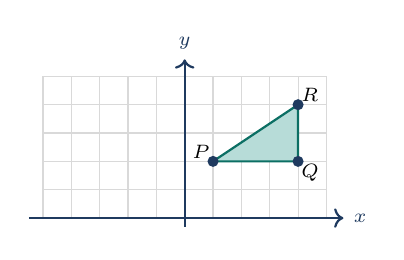
\begin{tikzpicture}[x=0.36cm,y=0.36cm]
\draw[gray!30,xstep=1,ystep=1] (-5,0) grid (5,5);
\draw[->,thick,mainc] (-5.5,0)--(5.6,0) node[right,font=\scriptsize]{$x$};
\draw[->,thick,mainc] (0,-0.3)--(0,5.6) node[above,font=\scriptsize]{$y$};
\fill[accc!30] (1,2)--(4,2)--(4,4)--cycle;
\draw[accc!80!black,thick] (1,2)--(4,2)--(4,4)--cycle;
\fill[mainc] (1,2) circle (2pt) (4,2) circle (2pt) (4,4) circle (2pt);
\node[font=\scriptsize,above left,inner sep=1pt] at (1,2) {$P$};
\node[font=\scriptsize,below right,inner sep=1pt] at (4,2) {$Q$};
\node[font=\scriptsize,above right,inner sep=1pt] at (4,4) {$R$};
\end{tikzpicture}}}{\pil{$(4,-4)$}{$(-4,-4)$}{$(4,4)$}{$(-2,4)$}{$(-4,4)$}}

\tingkat{Tingkat Sedang}{soal 6 sampai 10}
\soal{Diketahui $A=\begin{bmatrix}2&-1\\1&3\end{bmatrix}$. Jika $A^2-pA+qI=O$, nilai $p+q$ adalah \dots.}{\pil{$2$}{$7$}{$10$}{$12$}{$35$}}
\soal{\gbr{Dua cabang toko alat tulis menyimpan stok pena, buku, dan map seperti pada tabel. Harga satuan (dalam ribuan rupiah) adalah $8$, $5$, dan $12$. Jika semua harga naik $20\%$, selisih nilai persediaan Toko 2 dan Toko 1 adalah \dots.}{%
\small\renewcommand{\arraystretch}{1.25}
\begin{tabular}{@{}l|ccc@{}}
\textbf{Stok} & Pena & Buku & Map\\\hline
Toko 1 & $10$ & $20$ & $5$\\
Toko 2 & $15$ & $10$ & $10$\\\hline
\textbf{Harga} & $8$ & $5$ & $12$
\end{tabular}}}{\pil{Rp50.000}{Rp55.000}{Rp60.000}{Rp65.000}{Rp72.000}}
\soal{Matriks $A$ berordo $3\times3$ dengan $\det(A)=3$. Nilai $\det\!\big(2A^{2}(A^{T})^{-1}\big)$ adalah \dots.}{\pil{$6$}{$24$}{$12$}{$48$}{$72$}}
\soal{\gbr{Gambar menunjukkan grafik garis $g$ dan garis $h$. Sistem persamaan linear dari kedua garis ditulis $ax+by=e$ (garis $g$ lebih dulu, lalu $h$). Dengan aturan Cramer, nilai $D_x+D_y$ adalah \dots.}{%
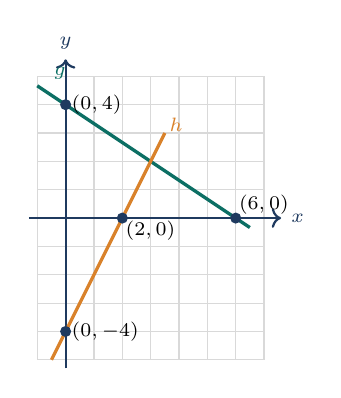
\begin{tikzpicture}[x=0.36cm,y=0.36cm]
\draw[gray!30,xstep=1,ystep=1] (-1,-5) grid (7,5);
\draw[->,thick,mainc] (-1.3,0)--(7.6,0) node[right,font=\scriptsize]{$x$};
\draw[->,thick,mainc] (0,-5.3)--(0,5.6) node[above,font=\scriptsize]{$y$};
\draw[accc!80!black,very thick] (-1,4.667)--(6.5,-0.333);
\draw[warmc,very thick] (-0.5,-5)--(3.5,3);
\fill[mainc] (6,0) circle (2pt) (0,4) circle (2pt) (2,0) circle (2pt) (0,-4) circle (2pt);
\node[font=\scriptsize,above right,inner sep=1pt] at (6,0) {$(6,0)$};
\node[font=\scriptsize,right,inner sep=2pt] at (0,4) {$(0,4)$};
\node[font=\scriptsize,below right,inner sep=1pt] at (2,0) {$(2,0)$};
\node[font=\scriptsize,right,inner sep=2pt] at (0,-4) {$(0,-4)$};
\node[font=\scriptsize,accc!80!black] at (-0.2,5.1) {$g$};
\node[font=\scriptsize,warmc] at (3.9,3.3) {$h$};
\end{tikzpicture}}}{\pil{$-48$}{$-24$}{$-8$}{$40$}{$-40$}}
\soal{\gbr{Gambar menunjukkan persegi satuan $OABC$ dan bayangannya $OA'B'C'$ oleh transformasi linear $T$. Bayangan titik $(2,3)$ oleh $T$ adalah \dots.}{%
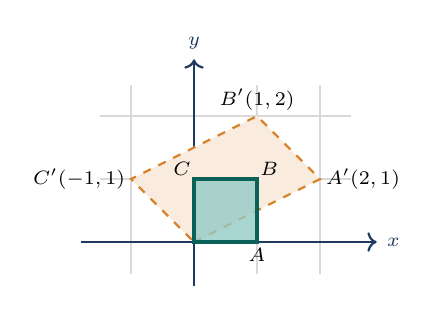
\begin{tikzpicture}[x=0.8cm,y=0.8cm]
\draw[gray!30,xstep=1,ystep=1] (-1.5,-0.5) grid (2.5,2.5);
\draw[->,thick,mainc] (-1.8,0)--(2.9,0) node[right,font=\scriptsize]{$x$};
\draw[->,thick,mainc] (0,-0.7)--(0,2.9) node[above,font=\scriptsize]{$y$};
\fill[warmc!15] (0,0)--(2,1)--(1,2)--(-1,1)--cycle;
\draw[warmc,thick,dashed] (0,0)--(2,1)--(1,2)--(-1,1)--cycle;
\fill[accc!45,fill opacity=0.8] (0,0)--(1,0)--(1,1)--(0,1)--cycle;
\draw[accc!70!black,very thick] (0,0)--(1,0)--(1,1)--(0,1)--cycle;
\node[font=\scriptsize,below,inner sep=2pt] at (1,0) {$A$};
\node[font=\scriptsize,above right,inner sep=1pt] at (1,1) {$B$};
\node[font=\scriptsize,above left,inner sep=1pt] at (0,1) {$C$};
\node[font=\scriptsize,right,inner sep=2pt] at (2,1) {$A'(2,1)$};
\node[font=\scriptsize,above,inner sep=2pt] at (1,2) {$B'(1,2)$};
\node[font=\scriptsize,left,inner sep=2pt] at (-1,1) {$C'(-1,1)$};
\end{tikzpicture}}}{\pilx{$(5,1)$}{$(-1,5)$}{$(7,1)$}{$(1,5)$}{$(4,2)$}}

\tingkat{Tingkat Sulit}{soal 11 sampai 15, setara UTBK}
\soal{Diketahui $A=\begin{bmatrix}3&1\\5&2\end{bmatrix}$ dan $B=\begin{bmatrix}1&2\\3&4\end{bmatrix}$. Jika matriks $X$ memenuhi $XA=B$, elemen baris kedua kolom pertama matriks $X$ adalah \dots.}{\pil{$-8$}{$4$}{$-14$}{$5$}{$9$}}
\soal{Sistem persamaan linear
$\begin{cases}x+y+z=6\\ x-y+2z=5\\ 4x+2y+az=b\end{cases}$
memiliki tak hingga banyak solusi. Nilai $a+b$ adalah \dots.}{\pil{$5$}{$28$}{$23$}{$18$}{$33$}}
\soal{\gbr{Segitiga $ABC$ pada gambar dipetakan oleh $T=\begin{bmatrix}2&k\\1&3\end{bmatrix}$ menjadi segitiga berluas $42$ satuan luas. Jumlah semua nilai $k$ yang mungkin adalah \dots.}{%
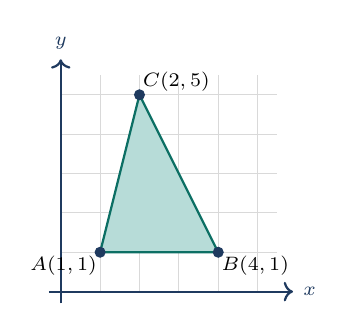
\begin{tikzpicture}[x=0.5cm,y=0.5cm]
\draw[gray!30,xstep=1,ystep=1] (0,0) grid (5.5,5.5);
\draw[->,thick,mainc] (-0.3,0)--(5.9,0) node[right,font=\scriptsize]{$x$};
\draw[->,thick,mainc] (0,-0.3)--(0,5.9) node[above,font=\scriptsize]{$y$};
\fill[accc!30] (1,1)--(4,1)--(2,5)--cycle;
\draw[accc!80!black,thick] (1,1)--(4,1)--(2,5)--cycle;
\fill[mainc] (1,1) circle (2pt) (4,1) circle (2pt) (2,5) circle (2pt);
\node[font=\scriptsize,below left,inner sep=1pt] at (1,1) {$A(1,1)$};
\node[font=\scriptsize,below right,inner sep=1pt] at (4,1) {$B(4,1)$};
\node[font=\scriptsize,above right,inner sep=1pt] at (2,5) {$C(2,5)$};
\end{tikzpicture}}}{\pil{$12$}{$13$}{$-13$}{$6$}{$14$}}
\soal{Diketahui $A=\begin{bmatrix}1&2\\0&1\end{bmatrix}$ dan $B=\begin{bmatrix}1&0\\3&1\end{bmatrix}$. Perhatikan pernyataan berikut.
\begin{enumerate}[label=(\arabic*),leftmargin=1.8em,itemsep=0pt,topsep=2pt]
\item $AB=BA$.
\item $\det(AB)=\det(BA)$.
\item $(AB)^T=A^TB^T$.
\item $AB-BA=\begin{bmatrix}6&0\\0&-6\end{bmatrix}$.
\end{enumerate}
Pernyataan yang benar adalah \dots.}{\begin{tabularx}{\linewidth}{@{}*{3}{X}@{}}\textbf{A.}\;(1) dan (2) saja & \textbf{B.}\;(1) dan (3) saja & \textbf{C.}\;(2) dan (4) saja\\[3pt] \textbf{D.}\;(1), (3), dan (4) saja & \textbf{E.}\;(2), (3), dan (4) saja & \end{tabularx}}
\soal{Diketahui $A=\begin{bmatrix}1&2&0\\3&1&2\\0&1&1\end{bmatrix}$. Elemen baris kedua kolom ketiga pada $A^{-1}$ adalah \dots.}{\pil{$\dis\frac17$}{$\dis-\frac27$}{$\dis-\frac17$}{$\dis\frac27$}{$\dis\frac37$}}

\tingkat{Tingkat HOTS}{soal 16 sampai 20, penalaran tingkat tinggi gaya UTBK}
\soal{\gbr{Diagram menunjukkan jalur satu arah antara empat kota $P$, $Q$, $R$, dan $S$. Banyak rute berbeda dengan tepat tiga ruas jalan yang berawal dan berakhir di kota yang sama (kota awalnya boleh $P$, $Q$, $R$, atau $S$) adalah \dots.\par\smallskip\footnotesize (Petunjuk: susun matriks ketetanggaan, yaitu elemen baris $i$ kolom $j$ bernilai $1$ jika ada jalur langsung dari kota $i$ ke kota $j$.)}{%
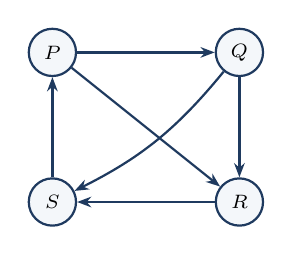
\begin{tikzpicture}[scale=0.95]
\node[nd] (P) at (0,2) {$P$}; \node[nd] (Q) at (2.5,2) {$Q$};
\node[nd] (R) at (2.5,0) {$R$}; \node[nd] (S) at (0,0) {$S$};
\draw[ar] (P)--(Q); \draw[ar] (Q)--(R); \draw[ar] (R)--(S); \draw[ar] (S)--(P);
\draw[ar] (P)--(R);
\draw[ar] (Q) to[bend left=12] (S);
\end{tikzpicture}}}{\pil{$0$}{$4$}{$5$}{$11$}{$6$}}
\soal{Apakah matriks $B=\begin{bmatrix}1&2&3\\4&5&6\\7&8&k\end{bmatrix}$ mempunyai invers?
\begin{enumerate}[label=(\arabic*),leftmargin=1.8em,itemsep=0pt,topsep=2pt]
\item $k=9$.
\item Jumlah elemen pada diagonal utama $B$ adalah $15$.
\end{enumerate}}{\begin{tabularx}{\linewidth}{@{}lX@{}}
\textbf{A.} & Pernyataan (1) SAJA cukup untuk menjawab pertanyaan, tetapi pernyataan (2) SAJA tidak cukup.\\
\textbf{B.} & Pernyataan (2) SAJA cukup untuk menjawab pertanyaan, tetapi pernyataan (1) SAJA tidak cukup.\\
\textbf{C.} & DUA pernyataan BERSAMA-SAMA cukup untuk menjawab pertanyaan, tetapi SATU pernyataan SAJA tidak cukup.\\
\textbf{D.} & Pernyataan (1) SAJA cukup dan pernyataan (2) SAJA cukup untuk menjawab pertanyaan.\\
\textbf{E.} & Pernyataan (1) dan pernyataan (2) tidak cukup untuk menjawab pertanyaan.
\end{tabularx}}
\soal{\gbr{Titik $P_k=M^k\begin{bmatrix}1\\0\end{bmatrix}$ untuk $k=0,1,\dots,5$ dengan $M=\begin{bmatrix}\cos60^\circ&-\sin60^\circ\\\sin60^\circ&\cos60^\circ\end{bmatrix}$ membentuk segienam beraturan pada gambar. Tentukan nilai kebenaran tiga pernyataan berikut (B = benar, S = salah), berurutan dari (i) sampai (iii).\par\smallskip
(i) $M^6=I$.\par
(ii) $M^2-M+I=O$.\par
(iii) $M^3=I$.}{%
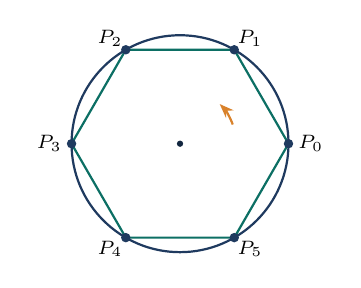
\begin{tikzpicture}[scale=0.95]
\def\R{1.45}
\draw[thick,mainc] (0,0) circle (\R);
\draw[accc!80!black,thick] (0:\R)--(60:\R)--(120:\R)--(180:\R)--(240:\R)--(300:\R)--cycle;
\foreach \k in {0,...,5}{\fill[mainc] (60*\k:\R) circle (1.8pt);}
\node[font=\scriptsize,right] at (0:\R) {$P_0$}; \node[font=\scriptsize,above right,inner sep=1pt] at (60:\R) {$P_1$};
\node[font=\scriptsize,above left,inner sep=1pt] at (120:\R) {$P_2$}; \node[font=\scriptsize,left] at (180:\R) {$P_3$};
\node[font=\scriptsize,below left,inner sep=1pt] at (240:\R) {$P_4$}; \node[font=\scriptsize,below right,inner sep=1pt] at (300:\R) {$P_5$};
\draw[ar,warmc] (20:0.75) arc (20:45:0.75);
\fill[deepc] (0,0) circle (1.2pt);
\end{tikzpicture}}}{\pilx{B, B, B}{B, B, S}{B, S, B}{S, B, B}{S, S, B}}
\soal{Matriks $A=\begin{bmatrix}a&b\\c&d\end{bmatrix}$ memenuhi $A^2=I$, $A\neq I$, dan $A\neq-I$. Nilai $a+d$ dan $ad-bc$ berturut-turut adalah \dots.}{\pilx{$0$ dan $-1$}{$0$ dan $1$}{$1$ dan $-1$}{$-1$ dan $0$}{$2$ dan $1$}}
\soal{\gbr{Penduduk kota $A$ dan $B$ berpindah mengikuti diagram: tiap tahun $20\%$ penduduk $A$ pindah ke $B$ dan $30\%$ penduduk $B$ pindah ke $A$, sedangkan sisanya menetap. Jumlah penduduk kedua kota selalu $1000$ jiwa. Pada keadaan setimbang (banyak penduduk tiap kota tidak berubah dari tahun ke tahun), penduduk kota $A$ berjumlah \dots\ jiwa.}{%
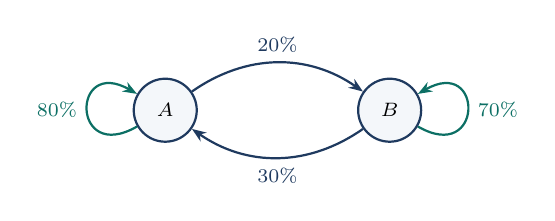
\begin{tikzpicture}[scale=0.95]
\node[nd,minimum size=8mm] (A) at (0,0) {$A$}; \node[nd,minimum size=8mm] (B) at (3,0) {$B$};
\draw[ar] (A) to[bend left=35] node[above,font=\scriptsize]{$20\%$} (B);
\draw[ar] (B) to[bend left=35] node[below,font=\scriptsize]{$30\%$} (A);
\draw[ar,accc!80!black] (A) to[out=210,in=150,looseness=6] node[left,font=\scriptsize]{$80\%$} (A);
\draw[ar,accc!80!black] (B) to[out=-30,in=30,looseness=6] node[right,font=\scriptsize]{$70\%$} (B);
\end{tikzpicture}}}{\pil{$500$}{$625$}{$600$}{$650$}{$700$}}

% =====================================================================
\bagian{B. Isian Singkat}{5 soal $\times$ 4 poin = 20 poin. Tuliskan hanya jawaban akhir.}

\tingkat{Tingkat Sedang}{soal 1 dan 2}
\soal{Diketahui $A=\begin{bmatrix}2&1\\-1&3\end{bmatrix}$ dan $B=\begin{bmatrix}1&0\\2&-1\end{bmatrix}$. Nilai $\det(AB-BA)$ adalah \dots.}{\jwb}
\soal{Titik $P(2,-1)$ dirotasikan $90^\circ$ berlawanan arah jarum jam terhadap titik asal, kemudian didilatasi dengan faktor $3$ terhadap titik asal, lalu dicerminkan terhadap sumbu-$x$. Koordinat bayangan akhir titik $P$ adalah \dots.}{\jwb}

\tingkat{Tingkat Sulit}{soal 3 sampai 5}
\soal{Diketahui $A=\begin{bmatrix}2&1\\0&2\end{bmatrix}$. Jumlah semua elemen matriks $A^{6}$ adalah \dots.}{\jwb}
\soal{\gbr{Matriks $M$ berordo $3\times3$ adalah persegi ajaib: jumlah elemen setiap baris, setiap kolom, dan kedua diagonal utamanya sama. Tiga elemennya sudah diketahui (lihat gambar), sedangkan elemen lain belum diketahui dan tidak harus bilangan bulat positif. Nilai $\det(M)$ adalah \dots.}{%
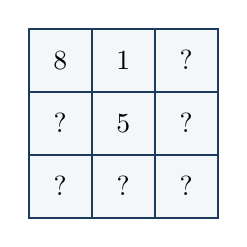
\begin{tikzpicture}
\foreach \r/\c/\t in {0/0/8,0/1/1,0/2/?,1/0/?,1/1/5,1/2/?,2/0/?,2/1/?,2/2/?}
  \node[draw=mainc,thick,minimum size=8mm,inner sep=0pt,fill=softbg] at (0.8*\c,-0.8*\r) {$\t$};
\end{tikzpicture}}}{\jwb}
\soal{\gbr{Graf tak berarah dengan lima titik pada gambar mempunyai matriks ketetanggaan $A$ (elemen $a_{ij}=1$ jika titik $i$ dan $j$ terhubung langsung, selain itu $0$). Nilai $\tr(A^3)$, yaitu jumlah elemen diagonal utama $A^3$, adalah \dots.}{%
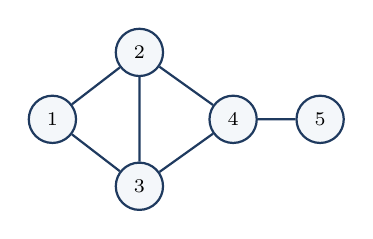
\begin{tikzpicture}[scale=0.85]
\node[nd] (1) at (0,1) {$1$}; \node[nd] (2) at (1.3,2) {$2$}; \node[nd] (3) at (1.3,0) {$3$};
\node[nd] (4) at (2.7,1) {$4$}; \node[nd] (5) at (4,1) {$5$};
\draw[thick,mainc] (1)--(2) (1)--(3) (2)--(3) (2)--(4) (3)--(4) (4)--(5);
\end{tikzpicture}}}{\jwb}

% =====================================================================
\Needspace{16\baselineskip}
\bagian{C. Uraian (Essay)}{5 soal $\times$ 8 poin = 40 poin. Tuliskan langkah penyelesaian dengan lengkap.}

\tingkat{Tingkat Sedang}{soal 1 dan 2}
\soal{\gbr{Segitiga $ABC$ dengan $A(1,1)$, $B(4,1)$, dan $C(1,3)$ pertama-tama dirotasikan $90^\circ$ berlawanan arah jarum jam terhadap titik asal (matriks $R$), kemudian didilatasi dengan faktor $2$ terhadap titik asal (matriks $D$).\par\smallskip
(a) Tentukan matriks $R$, matriks $D$, dan matriks komposisi $M$ yang memetakan $ABC$ langsung ke bayangan akhirnya.\par
(b) Tentukan koordinat $A'$, $B'$, dan $C'$.\par
(c) Hitung luas $A'B'C'$ dengan dua cara: dari koordinat dan dari $|\det M|$.\par
(d) Bayangan $A'B'C'$ lalu dicerminkan terhadap sumbu-$x$. Tentukan matriks komposisi barunya. Apakah luas berubah? Apa arti tanda determinan yang negatif?}{%
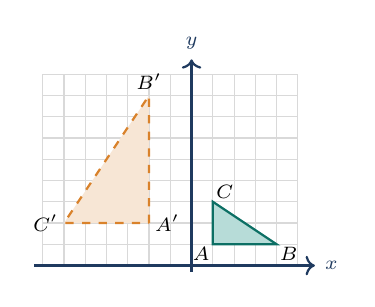
\begin{tikzpicture}[x=0.27cm,y=0.27cm]
\draw[gray!30,xstep=1,ystep=1] (-7,0) grid (5,9);
\draw[->,thick,mainc] (-7.4,0)--(5.8,0) node[right,font=\scriptsize]{$x$};
\draw[->,thick,mainc] (0,-0.3)--(0,9.7) node[above,font=\scriptsize]{$y$};
\fill[accc!30] (1,1)--(4,1)--(1,3)--cycle;
\draw[accc!80!black,thick] (1,1)--(4,1)--(1,3)--cycle;
\fill[warmc!20] (-2,2)--(-2,8)--(-6,2)--cycle;
\draw[warmc,thick,dashed] (-2,2)--(-2,8)--(-6,2)--cycle;
\node[font=\scriptsize,below left,inner sep=1pt] at (1,1) {$A$}; \node[font=\scriptsize,below right,inner sep=1pt] at (4,1) {$B$};
\node[font=\scriptsize,above right,inner sep=1pt] at (1,3) {$C$};
\node[font=\scriptsize,right,inner sep=2pt] at (-2,2) {$A'$}; \node[font=\scriptsize,above,inner sep=2pt] at (-2,8) {$B'$};
\node[font=\scriptsize,left,inner sep=2pt] at (-6,2) {$C'$};
\end{tikzpicture}}}{\poin{8}}
\soal{Seorang petani mencampur tiga jenis pupuk. Kandungan tiap kilogram pupuk (dalam gram) adalah: pupuk $X$ mengandung N $30$, P $10$, K $20$; pupuk $Y$ mengandung N $10$, P $20$, K $10$; pupuk $Z$ mengandung N $20$, P $10$, K $30$. Tanaman membutuhkan tepat N $280$ gram, P $210$ gram, dan K $290$ gram. Misalkan banyak pupuk $X$, $Y$, dan $Z$ (dalam kg) berturut-turut $x$, $y$, dan $z$.\par\smallskip
(a) Susun sistem persamaan linear yang paling sederhana dan tuliskan dalam bentuk $AX=B$.\par
(b) Hitung $\det(A)$ dan jelaskan arti nilainya terhadap banyaknya solusi.\par
(c) Tentukan $x$, $y$, dan $z$ dengan operasi baris elementer pada matriks augmented.\par
(d) Harga pupuk $X$, $Y$, dan $Z$ berturut-turut Rp12.000, Rp9.000, dan Rp15.000 per kg. Hitung biaya total campuran tersebut dengan perkalian matriks.}{\poin{8}}

\tingkat{Tingkat Sulit}{soal 3 dan 4}
\soal{Diketahui $A=\begin{bmatrix}2&1\\1&2\end{bmatrix}$.\par\smallskip
(a) Tunjukkan bahwa $A^2-4A+3I=O$.\par
(b) Dari persamaan pada (a) saja (tanpa rumus invers $2\times2$), nyatakan $A^{-1}$ dalam $A$ dan $I$, lalu hitung $A^{-1}$.\par
(c) Buktikan $A^3=13A-12I$, lalu hitung $A^3$.\par
(d) Tunjukkan bahwa $A^n=\dfrac{3^n-1}{2}A-\dfrac{3^n-3}{2}I$ berlaku untuk $n=2$ dan $n=3$, lalu gunakan rumus itu untuk menghitung $A^5$.}{\poin{8}}
\soal{\gbr{Dua vektor $\vec u=\begin{bmatrix}4\\1\end{bmatrix}$ dan $\vec v=\begin{bmatrix}1\\3\end{bmatrix}$ membentuk jajargenjang $OUWV$ (lihat gambar). Matriks $T$ memetakan persegi satuan menjadi jajargenjang tersebut: $\begin{bmatrix}1\\0\end{bmatrix}\mapsto\vec u$ dan $\begin{bmatrix}0\\1\end{bmatrix}\mapsto\vec v$.\par\smallskip
(a) Tentukan $T$ dan luas jajargenjang $OUWV$.\par
(b) Tentukan $T^{-1}$.\par
(c) Titik $P\left(\frac52,2\right)$ dapat ditulis $\overrightarrow{OP}=s\vec u+t\vec v$. Tentukan $(s,t)$ dengan $T^{-1}$ dan jelaskan letak $P$ pada jajargenjang.\par
(d) Sebuah daerah $F$ di dalam jajargenjang berluas $3{,}3$ satuan luas. Berapa luas daerah asalnya di dalam persegi satuan? Jelaskan.}{%
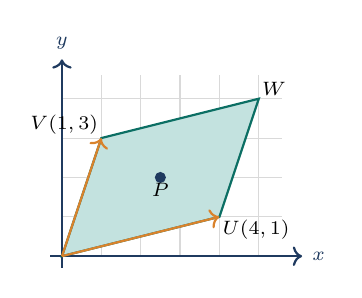
\begin{tikzpicture}[x=0.5cm,y=0.5cm]
\draw[gray!30,xstep=1,ystep=1] (0,0) grid (5.6,4.6);
\draw[->,thick,mainc] (-0.3,0)--(6.1,0) node[right,font=\scriptsize]{$x$};
\draw[->,thick,mainc] (0,-0.3)--(0,5) node[above,font=\scriptsize]{$y$};
\fill[accc!25] (0,0)--(4,1)--(5,4)--(1,3)--cycle;
\draw[accc!80!black,thick] (0,0)--(4,1)--(5,4)--(1,3)--cycle;
\draw[->,thick,warmc] (0,0)--(4,1); \draw[->,thick,warmc] (0,0)--(1,3);
\fill[mainc] (2.5,2) circle (2pt);
\node[font=\scriptsize,below right,inner sep=1pt] at (4,1) {$U(4,1)$};
\node[font=\scriptsize,above right,inner sep=1pt] at (5,4) {$W$};
\node[font=\scriptsize,above left,inner sep=1pt] at (1,3) {$V(1,3)$};
\node[font=\scriptsize,below,inner sep=2pt] at (2.5,2) {$P$};
\end{tikzpicture}}}{\poin{8}}

\tingkat{Tingkat HOTS}{soal 5}
\soal{Sandi Hill mengubah huruf menjadi angka (lihat tabel), lalu mengenkripsi pasangan huruf dengan matriks kunci $K$: pasangan $\begin{bmatrix}p_1\\p_2\end{bmatrix}$ menjadi $\begin{bmatrix}c_1\\c_2\end{bmatrix}\equiv K\begin{bmatrix}p_1\\p_2\end{bmatrix}\pmod{26}$. Notasi $a\bmod 26$ berarti sisa pembagian $a$ oleh $26$ (misalnya $33\bmod26=7$). Pada soal ini $K=\begin{bmatrix}3&3\\2&5\end{bmatrix}$. Untuk mendekripsi dipakai $K^{-1}$ yang memenuhi $KK^{-1}\equiv I\pmod{26}$.\par\smallskip
\begin{center}\small\renewcommand{\arraystretch}{1.1}\setlength{\tabcolsep}{3pt}
\begin{tabular}{|*{13}{c|}}\hline
A&B&C&D&E&F&G&H&I&J&K&L&M\\\hline
0&1&2&3&4&5&6&7&8&9&10&11&12\\\hline\hline
N&O&P&Q&R&S&T&U&V&W&X&Y&Z\\\hline
13&14&15&16&17&18&19&20&21&22&23&24&25\\\hline
\end{tabular}\end{center}\vspace{-0.3em}
(a) Enkripsikan kata \textbf{HELP}.\par
(b) Tunjukkan $K$ dapat didekripsi: hitung $\det(K)$, cari $u$ dengan $9u\equiv1\pmod{26}$, lalu tentukan $K^{-1}$ modulo $26$ dengan $K^{-1}\equiv u\cdot\adj(K)$.\par
(c) Dekripsikan pesan \textbf{LDXKBU}.\par
(d) Kunci $K'=\begin{bmatrix}4&1\\2&3\end{bmatrix}$ memiliki $\det(K')\neq0$, tetapi tidak dapat dipakai. Tunjukkan dua pasangan huruf berbeda yang menghasilkan sandi sama, lalu simpulkan syarat $\det(K)$ agar kunci layak dipakai.}{\poin{8}}

% =====================================================================
\newpage
\bagian{Kunci Jawaban dan Pembahasan Singkat}{Untuk guru dan pembahasan mandiri}
\par\vspace{0.6em}{\bfseries\color{mainc}Kunci Pilihan Ganda}\par\vspace{0.3em}
\small
\begin{tabularx}{\linewidth}{@{}*{10}{>{\centering\arraybackslash}X}@{}}\hline \textbf{1} & \textbf{2} & \textbf{3} & \textbf{4} & \textbf{5} & \textbf{6} & \textbf{7} & \textbf{8} & \textbf{9} & \textbf{10}\\ \hline C & B & D & A & E & D & C & B & E & D\\ \hline\end{tabularx}\\[6pt]
\begin{tabularx}{\linewidth}{@{}*{10}{>{\centering\arraybackslash}X}@{}}\hline \textbf{11} & \textbf{12} & \textbf{13} & \textbf{14} & \textbf{15} & \textbf{16} & \textbf{17} & \textbf{18} & \textbf{19} & \textbf{20}\\ \hline C & B & A & C & D & E & D & B & A & C\\ \hline\end{tabularx}
\par\vspace{0.8em}{\bfseries\color{mainc}\normalsize Pembahasan Pilihan Ganda}\par\vspace{0.2em}
\small\begin{enumerate}[leftmargin=2em,itemsep=2pt,topsep=2pt]
\item[\textbf{1.}] \textbf{(C)} $p_{23}=2(2)-3=1$ dan $p_{34}=2(3)-4=2$, sehingga jumlahnya $3$. (Jebakan: tertukar $i$ dan $j$.)
\item[\textbf{2.}] \textbf{(B)} Kesamaan matriks: $x+2y=8$ dan $2x-y=1$. Dari persamaan kedua $y=2x-1$, sehingga $x+4x-2=8\Rightarrow x=2$, $y=3$. Maka $xy=6$.
\item[\textbf{3.}] \textbf{(D)} $B^T=\sm{0&-1\\1&2}$ dan $2A=\sm{2&-4\\6&8}$, sehingga $2A-B^T=\sm{2&-3\\5&6}$. (Jebakan A: lupa men-transpose $B$; B: salah mengurangi menjadi menjumlah.)
\item[\textbf{4.}] \textbf{(A)} $\det=5\cdot3-2\cdot7=1$. Tukar $a$ dan $d$, ubah tanda $b$ dan $c$: $A^{-1}=\sm{3&-2\\-7&5}$. (Jebakan E: transpose, bukan tukar-tanda.)
\item[\textbf{5.}] \textbf{(E)} Bayangan $(x,y)$ adalah $(-x,y)$, jadi $R(4,4)\to R'(-4,4)$.
\item[\textbf{6.}] \textbf{(D)} Menurut teorema Cayley--Hamilton, $p=\tr(A)=5$ dan $q=\det(A)=7$. Verifikasi: $A^2=\sm{3&-5\\5&8}$ dan $A^2-5A+7I=O$. Jadi $p+q=12$. (Jebakan $35$: $pq$.)
\item[\textbf{7.}] \textbf{(C)} Nilai persediaan $=S\cdot h=\begin{bmatrix}10&20&5\\15&10&10\end{bmatrix}\begin{bmatrix}8\\5\\12\end{bmatrix}=\begin{bmatrix}240\\290\end{bmatrix}$ (ribuan rupiah). Selisih $50$, setelah naik $20\%$ menjadi $1{,}2\times50=60$ ribu, yaitu Rp60.000.
\item[\textbf{8.}] \textbf{(B)} Untuk matriks $3\times3$, $\det(kM)=k^3\det M$. Maka $\det(2A^2(A^T)^{-1})=2^3\cdot(\det A)^2\cdot\dfrac1{\det A}=8\cdot9\cdot\dfrac13=24$. (Jebakan A: memakai faktor $2$, bukan $2^3$.)
\item[\textbf{9.}] \textbf{(E)} Garis $g$ melalui $(6,0)$ dan $(0,4)$: $2x+3y=12$. Garis $h$ melalui $(2,0)$ dan $(0,-4)$: $2x-y=4$. $D=\begin{vmatrix}2&3\\2&-1\end{vmatrix}=-8$, $D_x=\begin{vmatrix}12&3\\4&-1\end{vmatrix}=-24$, $D_y=\begin{vmatrix}2&12\\2&4\end{vmatrix}=-16$. Jadi $D_x+D_y=-40$. (Cek: $x=\frac{-24}{-8}=3$, $y=2$.) Jebakan A: ikut menjumlahkan $D$.
\item[\textbf{10.}] \textbf{(D)} Kolom matriks $T$ adalah bayangan vektor basis: $T=\sm{2&-1\\1&1}$. Maka $T\begin{bmatrix}2\\3\end{bmatrix}=\begin{bmatrix}4-3\\2+3\end{bmatrix}=(1,5)$. Kolom pertama adalah bayangan $A(1,0)$ dan kolom kedua bayangan $C(0,1)$.
\item[\textbf{11.}] \textbf{(C)} $XA=B\Rightarrow X=BA^{-1}$ (invers dikalikan dari kanan). $A^{-1}=\sm{2&-1\\-5&3}$, sehingga $X=\sm{1&2\\3&4}\sm{2&-1\\-5&3}=\sm{-8&5\\-14&9}$ dan $x_{21}=-14$. (Jebakan B: memakai $A^{-1}B$, hasilnya $x_{21}=4$.)
\item[\textbf{12.}] \textbf{(B)} Baris pertama dan kedua dikombinasikan: $3R_1+R_2=4x+2y+5z=23$. Agar baris ketiga bergantung pada dua baris lain (tak hingga solusi), $a=5$ dan $b=23$. Jadi $a+b=28$. Cek: $\det\sm{1&1&1\\1&-1&2\\4&2&5}=0$. Jika $a=5$ tetapi $b\neq23$, sistem tidak punya solusi.
\item[\textbf{13.}] \textbf{(A)} Luas $ABC=\frac12\cdot3\cdot4=6$. $\det T=6-k$ dan luas bayangan $=|6-k|\cdot6=42\Rightarrow|6-k|=7$, sehingga $k=-1$ atau $k=13$. Jumlahnya $12$.
\item[\textbf{14.}] \textbf{(C)} $AB=\sm{7&2\\3&1}$ dan $BA=\sm{1&2\\3&7}$, sehingga (1) salah dan (4) benar karena $AB-BA=\sm{6&0\\0&-6}$. (2) benar karena $\det(AB)=\det A\det B=\det(BA)=1$. (3) salah: $(AB)^T=\sm{7&3\\2&1}=B^TA^T$, sedangkan $A^TB^T=\sm{1&3\\2&7}$.
\item[\textbf{15.}] \textbf{(D)} $\det A=1(1-2)-2(3-0)=-7$. $(A^{-1})_{23}=\dfrac{C_{32}}{\det A}$ (adjoin adalah transpose kofaktor). $C_{32}=-\begin{vmatrix}1&0\\3&2\end{vmatrix}=-2$, sehingga hasilnya $\dfrac{-2}{-7}=\dfrac27$. (Jebakan A: memakai $C_{23}=-1$ tanpa transpose.)
\item[\textbf{16.}] \textbf{(E)} Dengan urutan $P,Q,R,S$: $A=\sm{0&1&1&0\\0&0&1&1\\0&0&0&1\\1&0&0&0}$. Elemen diagonal $A^3$ menghitung rute tertutup tiga ruas: $P$: $PQSP$ dan $PRSP$ ($2$); $Q$: $QSPQ$ ($1$); $R$: $RSPR$ ($1$); $S$: $SPQS$ dan $SPRS$ ($2$). Total $\tr(A^3)=2+1+1+2=6$. (Jebakan $11$: jumlah semua elemen $A^3$.)
\item[\textbf{17.}] \textbf{(D)} $\det B=1(5k-48)-2(4k-42)+3(32-35)=27-3k=3(9-k)$. $B$ punya invers jika dan hanya jika $k\neq9$. Pernyataan (1): $k=9$, $\det B=0$, jawabannya \emph{tidak}. Pernyataan (2): $1+5+k=15\Rightarrow k=9$, jawabannya juga \emph{tidak}. Masing-masing cukup.
\item[\textbf{18.}] \textbf{(B)} $M$ adalah rotasi $60^\circ$ sehingga $M^k$ adalah rotasi $60k^\circ$. (i) $M^6$ rotasi $360^\circ=I$: \textbf{B}. (ii) $\tr(M)=1$ dan $\det M=1$, sehingga menurut Cayley--Hamilton $M^2-M+I=O$: \textbf{B} (cek langsung: $M^2-M=-I$). (iii) $M^3$ rotasi $180^\circ$ yaitu $-I\neq I$: \textbf{S}. Urutan: B, B, S.
\item[\textbf{19.}] \textbf{(A)} Cayley--Hamilton: $A^2-(a+d)A+(ad-bc)I=O$. Dengan $A^2=I$: $(a+d)A=(1+ad-bc)I$. Karena $A$ bukan matriks skalar ($A\neq\pm I$ dan $A^2=I$ memaksa diagonal skalar hanya $\pm I$), haruslah $a+d=0$ dan $1+ad-bc=0$, yaitu $ad-bc=-1$. Contoh: $A=\sm{1&0\\0&-1}$.
\item[\textbf{20.}] \textbf{(C)} Keadaan setimbang memenuhi $TX=X$ dengan $T=\sm{0{,}8&0{,}3\\0{,}2&0{,}7}$, yaitu $-0{,}2a+0{,}3b=0\Rightarrow b=\frac23a$. Dengan $a+b=1000$: $a+\frac23a=1000\Rightarrow a=600$ dan $b=400$. Cek: $0{,}8(600)+0{,}3(400)=600$. (Jebakan: $625$ adalah keadaan tahun ke-2 dari $(700,300)$.)
\end{enumerate}
\par\Needspace{6\baselineskip}\vspace{0.6em}{\bfseries\color{mainc}\normalsize Pembahasan Isian Singkat}\par\vspace{0.2em}
\small\begin{enumerate}[leftmargin=2em,itemsep=2pt,topsep=2pt]
\item[\textbf{1.}] \textbf{Jawaban: $-4$.} $AB=\sm{4&-1\\5&-3}$ dan $BA=\sm{2&1\\5&-1}$, sehingga $AB-BA=\sm{2&-2\\0&-2}$ dan determinannya $-4-0=-4$.
\item[\textbf{2.}] \textbf{Jawaban: $(3,-6)$.} Rotasi $90^\circ$: $(x,y)\to(-y,x)$, sehingga $(2,-1)\to(1,2)$. Dilatasi $3$: $(3,6)$. Cermin sumbu-$x$: $(3,-6)$. Matriks komposisi (urutan dari kanan): $\sm{1&0\\0&-1}\sm{3&0\\0&3}\sm{0&-1\\1&0}=\sm{0&-3\\-3&0}$.
\item[\textbf{3.}] \textbf{Jawaban: $320$.} Tulis $A=2I+N$ dengan $N=\sm{0&1\\0&0}$ dan $N^2=O$. Maka $A^n=2^nI+n2^{n-1}N$, sehingga $A^6=\sm{64&192\\0&64}$. Jumlah elemen $64+192+0+64=320$.
\item[\textbf{4.}] \textbf{Jawaban: $-360$.} Persegi ajaib $3\times3$ berbentuk $\sm{c+x&c-x-y&c+y\\c-x+y&c&c+x-y\\c-y&c+x+y&c-x}$. Dari $c=5$, $c+x=8$, dan $c-x-y=1$ diperoleh $x=3$ dan $y=1$, sehingga $M=\sm{8&1&6\\3&5&7\\4&9&2}$. Dengan Sarrus: $\det M=(8\cdot5\cdot2+1\cdot7\cdot4+6\cdot3\cdot9)-(6\cdot5\cdot4+8\cdot7\cdot9+1\cdot3\cdot2)=(80+28+162)-(120+504+6)=270-630=-360$.
\item[\textbf{5.}] \textbf{Jawaban: $12$.} Elemen diagonal $(A^3)_{ii}$ menghitung jalan tertutup tiga langkah dari titik $i$, yaitu segitiga yang memuat $i$ (dihitung dua arah). Graf memiliki $2$ segitiga ($1\text{-}2\text{-}3$ dan $2\text{-}3\text{-}4$), tiap segitiga memberi $6$ ($3$ titik awal $\times$ $2$ arah). Maka $\tr(A^3)=6\times2=12$. Pemeriksaan langsung: diagonal $A^3$ adalah $2,4,4,2,0$.
\end{enumerate}
\par\Needspace{8\baselineskip}\vspace{0.6em}{\bfseries\color{mainc}\normalsize Pembahasan dan Pedoman Penskoran Uraian}\par\vspace{0.2em}
\small\begin{enumerate}[leftmargin=2em,itemsep=3pt,topsep=2pt]
\item[\textbf{1.}] (a) $R=\sm{0&-1\\1&0}$, $D=\sm{2&0\\0&2}$, dan $M=DR=\sm{0&-2\\2&0}$ (urutan: rotasi lebih dulu sehingga $R$ berada di kanan). (b) $A'=M\sm{1\\1}=(-2,2)$, $B'=M\sm{4\\1}=(-2,8)$, $C'=M\sm{1\\3}=(-6,2)$. (c) Luas $ABC=\frac12\cdot3\cdot2=3$. Luas $A'B'C'$ dari koordinat: alas $A'B'=6$ (vertikal) dan tinggi jarak horizontal $C'$ ke garis $x=-2$ yaitu $4$, sehingga $\frac12\cdot6\cdot4=12$. Dari determinan: $\det M=0\cdot0-(-2)(2)=4$ dan $4\times3=12$. Keduanya sama. (d) $M_2=\sm{1&0\\0&-1}M=\sm{0&-2\\-2&0}$ dengan $\det M_2=-4$. Luas tetap $|{-4}|\times3=12$. Tanda negatif berarti orientasi bangun terbalik (urutan titik $A,B,C$ berubah dari berlawanan arah jarum jam menjadi searah), sedangkan besar luas ditentukan oleh $|\det|$. \\ \textit{Penskoran: tiap bagian 2 poin.}
\item[\textbf{2.}] (a) Persamaan: $30x+10y+20z=280$ disederhanakan menjadi $3x+y+2z=28$; $10x+20y+10z=210\Rightarrow x+2y+z=21$; $20x+10y+30z=290\Rightarrow2x+y+3z=29$. Bentuk $AX=B$: $\sm{3&1&2\\1&2&1\\2&1&3}\sm{x\\y\\z}=\sm{28\\21\\29}$. (b) $\det A=3(6-1)-1(3-2)+2(1-4)=15-1-6=8\neq0$, sehingga $A$ punya invers dan sistem memiliki \emph{tepat satu} solusi. (c) Augmented $\left[\begin{array}{ccc|c}1&2&1&21\\3&1&2&28\\2&1&3&29\end{array}\right]$ (baris disusun ulang agar elemen pertama $R_1$ bernilai $1$). $R_2\to R_2-3R_1$: $[0\ \,-5\ \,-1\,|\,-35]$; $R_3\to R_3-2R_1$: $[0\ \,-3\ \ 1\,|\,-13]$. Dari $R_3$: $z=3y-13$. Substitusi ke $R_2$: $-5y-(3y-13)=-35\Rightarrow-8y=-48\Rightarrow y=6$, sehingga $z=5$, dan $x=21-12-5=4$. Jadi $x=4$ kg, $y=6$ kg, $z=5$ kg. (d) Biaya $=\begin{bmatrix}4&6&5\end{bmatrix}\begin{bmatrix}12.000\\9.000\\15.000\end{bmatrix}=48.000+54.000+75.000=\text{Rp}177.000$. \\ \textit{Penskoran: (a) 2 poin; (b) 2 poin; (c) 3 poin; (d) 1 poin.}
\item[\textbf{3.}] (a) $A^2=\sm{5&4\\4&5}$, sehingga $A^2-4A+3I=\sm{5-8+3&4-4\\4-4&5-8+3}=O$. (b) Dari (a): $A^2-4A=-3I\Rightarrow A(A-4I)=-3I\Rightarrow A\cdot\dfrac{4I-A}{3}=I$. Jadi $A^{-1}=\dfrac13(4I-A)=\dfrac13\sm{2&-1\\-1&2}=\sm{\frac23&-\frac13\\-\frac13&\frac23}$. (c) $A^2=4A-3I$, sehingga $A^3=A\cdot A^2=4A^2-3A=4(4A-3I)-3A=13A-12I$. Hasil: $\sm{26-12&13\\13&26-12}=\sm{14&13\\13&14}$ (cek langsung $A\cdot A^2=\sm{14&13\\13&14}$). (d) $n=2$: $\frac{9-1}2A-\frac{9-3}2I=4A-3I$ (sama dengan (b)). $n=3$: $\frac{27-1}2A-\frac{27-3}2I=13A-12I$ (sama dengan (c)). Rumus untuk $n=5$: $\frac{243-1}2A-\frac{243-3}2I=121A-120I=\sm{242-120&121\\121&242-120}=\sm{122&121\\121&122}$. \\ \textit{Penskoran: (a) 1 poin; (b) 3 poin; (c) 2 poin; (d) 2 poin.}
\item[\textbf{4.}] (a) $T=\sm{4&1\\1&3}$ dan luas $=|\det T|=12-1=11$ satuan luas. (b) $T^{-1}=\dfrac1{11}\sm{3&-1\\-1&4}$. (c) $\sm{s\\t}=T^{-1}\sm{5/2\\2}=\dfrac1{11}\sm{15/2-2\\-5/2+8}=\sm{1/2\\1/2}$. Karena $s=t=\frac12$, $P=\frac12(\vec u+\vec v)$ adalah titik tengah diagonal $OW$, yaitu pusat jajargenjang (titik potong kedua diagonal). (d) $T$ mengalikan luas dengan $|\det T|=11$. Luas daerah asal $=\dfrac{3{,}3}{11}=0{,}3$ satuan luas, yaitu bayangan dengan $T^{-1}$ memperkecil luas dengan faktor $\frac1{11}$. \\ \textit{Penskoran: tiap bagian 2 poin.}
\item[\textbf{5.}] (a) $H=7$, $E=4$, $L=11$, $P=15$. Pasangan $(7,4)$: $K\sm{7\\4}=\sm{21+12\\14+20}=\sm{33\\34}\equiv\sm{7\\8}$, yaitu \textbf{HI}. Pasangan $(11,15)$: $\sm{33+45\\22+75}=\sm{78\\97}\equiv\sm{0\\19}$, yaitu \textbf{AT}. Jadi HELP $\to$ \textbf{HIAT}. (b) $\det K=15-6=9$. $9\cdot3=27\equiv1\pmod{26}$, sehingga $u=3$. $\adj(K)=\sm{5&-3\\-2&3}$, sehingga $K^{-1}\equiv3\sm{5&-3\\-2&3}=\sm{15&-9\\-6&9}\equiv\sm{15&17\\20&9}\pmod{26}$. Verifikasi: $K\cdot K^{-1}=\sm{105&78\\130&79}\equiv\sm{1&0\\0&1}$. (c) $LD=(11,3)$: $\sm{15\cdot11+17\cdot3\\20\cdot11+9\cdot3}=\sm{216\\247}\equiv\sm{8\\13}$, yaitu \textbf{IN}. $XK=(23,10)$: $\sm{345+170\\460+90}=\sm{515\\550}\equiv\sm{21\\4}$, yaitu \textbf{VE}. $BU=(1,20)$: $\sm{15+340\\20+180}=\sm{355\\200}\equiv\sm{17\\18}$, yaitu \textbf{RS}. Pesan: \textbf{INVERS}. (d) $\det K'=12-2=10$. Pasangan \textbf{AA} $(0,0)$ dan \textbf{NA} $(13,0)$: $K'\sm{13\\0}=\sm{52\\26}\equiv\sm{0\\0}$, sehingga keduanya menghasilkan sandi \textbf{AA} dan pesan tidak dapat didekripsi secara tunggal. Penyebab: $\gcd(10,26)=2\neq1$ sehingga $10$ tidak punya invers modulo $26$ dan $K'^{-1}$ modulo $26$ tidak ada. Syarat kunci layak: $\gcd(\det K,26)=1$, yaitu $\det K$ bukan kelipatan $2$ dan bukan kelipatan $13$. \\ \textit{Penskoran: (a) 2 poin; (b) 2 poin; (c) 2 poin; (d) 2 poin (contoh 1, kesimpulan syarat 1).}
\end{enumerate}
\end{document}
